% ============================================================================
% Chapter 01: Mathematical Preliminaries
% Part I: Foundations
% ============================================================================
% Purpose: Build physical intuition for differential geometry and quantum
%          formalism through real-world examples, establishing mathematical
%          language for unified field theory in whitepaper narrative style.
% ============================================================================

\chapter{Mathematical Preliminaries: The Language of Curved Spacetime}
\label{ch:prelim}
\index{mathematical preliminaries}
\index{curved spacetime}

%-----------------------------------------------------------------------------
% OPENING NARRATIVE: The GPS Paradox
%-----------------------------------------------------------------------------

\section*{The GPS Paradox}

Every time you use GPS navigation, your phone performs a calculation Einstein would have found miraculous: it accounts for the warping of time itself. Satellite clocks in GPS orbit tick approximately \SI{38}{\micro\second} faster per day than identical atomic clocks on Earth's surface. This is not experimental error---it is the direct consequence of general relativity\index{general relativity}\index{GPS!gravitational corrections} in action.

Without corrections for gravitational time dilation\index{time dilation!gravitational}\index{gravitational time dilation}, GPS would accumulate positioning errors of \SI{11}{\kilo\meter} per day. The system would be useless within hours. Engineers designing the GPS constellation in the 1970s had to program Einstein's equations into the satellites, making relativity essential to everyday technology.

Why does time flow differently at different altitudes? Because spacetime near Earth is curved by its mass. The GPS satellite at \SI{20200}{\kilo\meter} altitude experiences weaker gravitational curvature than a receiver on the ground. Clocks measure the geometry of spacetime itself, and that geometry is not flat.

% REMOVED nested figure wrapper - fig_gps_analogy.tex already contains complete figure environment
% \begin{figure}[h]
%   \centering
  %==============================================================================
% Figure: GPS Satellite Spacetime Curvature Analogy
% Purpose: Motivational diagram illustrating practical importance of GR
% Chapter: Ch01 - Mathematical Preliminaries (Opening)
% Type: Conceptual diagram / Real-world application
%==============================================================================

\begin{figure}[htbp]
  \centering
  \resizebox{\textwidth}{!}{%
  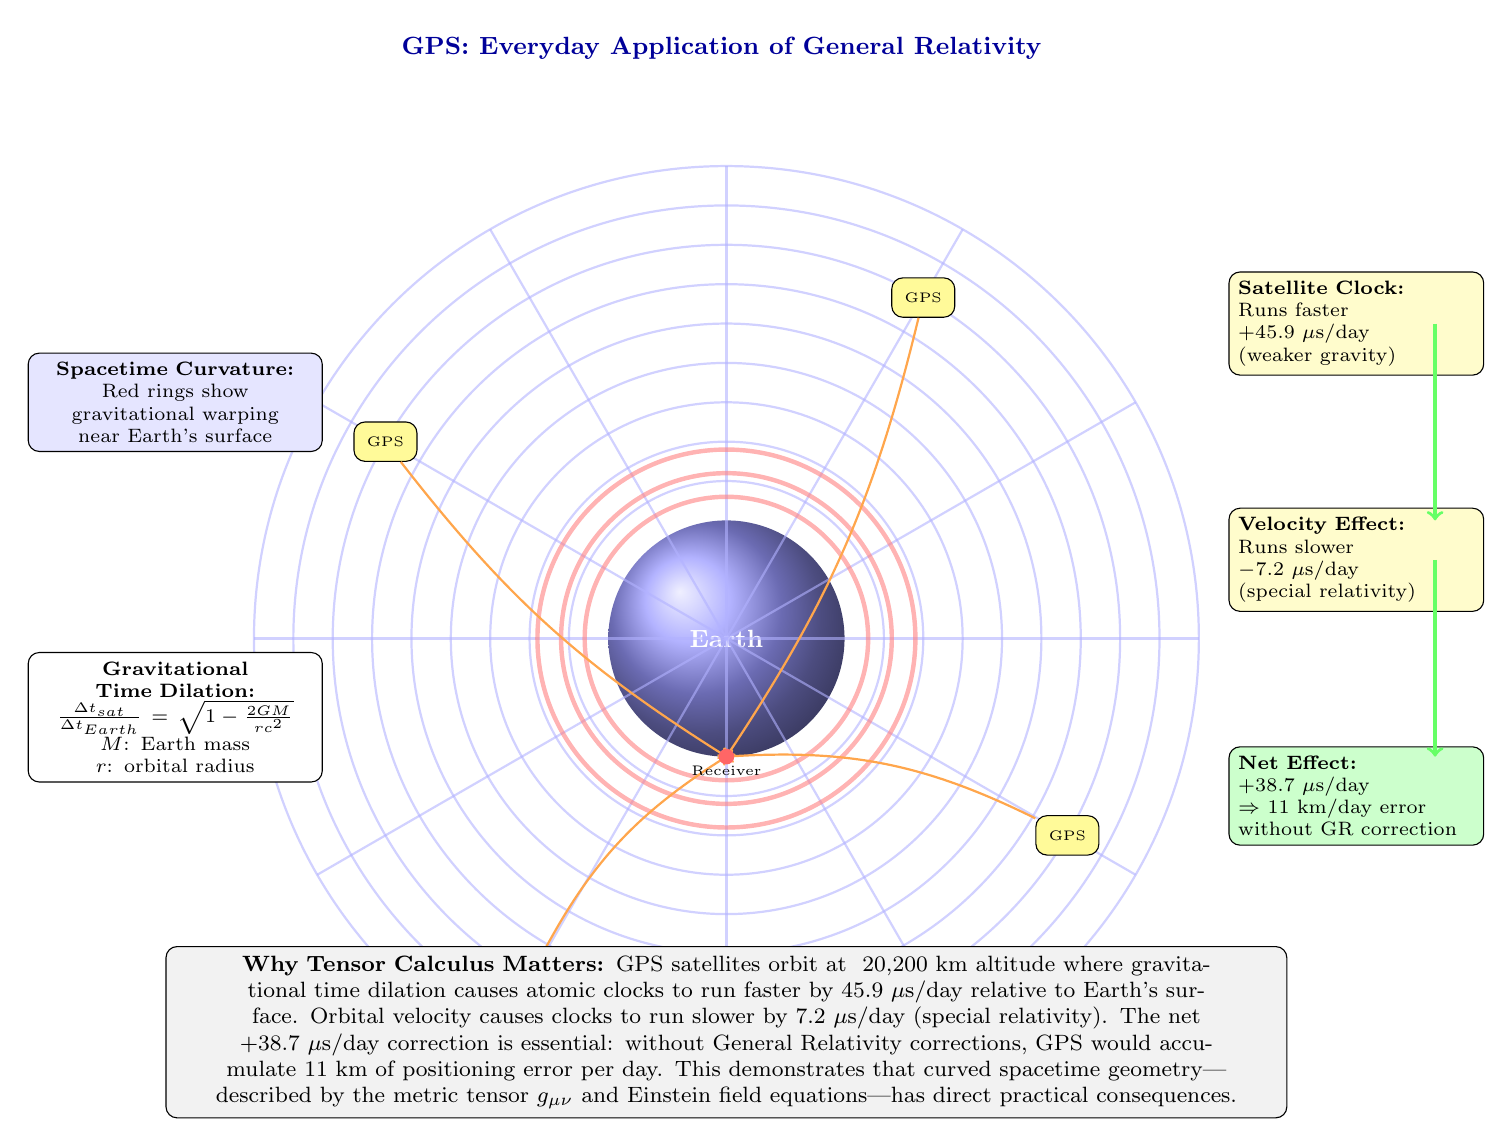
\begin{tikzpicture}[
    scale=1.0,
    satellite/.style={
      rectangle,
      rounded corners,
      minimum width=0.8cm,
      minimum height=0.5cm,
      draw=black,
      fill=gray!30,
      font=\tiny
    }
  ]

    % Earth (center)
    \shade[ball color=blue!40] (0,0) circle (1.5);
    \node[font=\small\bfseries, text=white] at (0,0) {Earth};

    % Spacetime curvature grid (warped by Earth's mass)
    % Background grid showing curvature
    \begin{scope}[opacity=0.6]
      % Curved grid lines (latitude-like)
      \foreach \r in {2, 2.5, 3, 3.5, 4, 4.5, 5, 5.5, 6} {
        \draw[blue!30, thick] (0,0) circle (\r);
      }

      % Curved grid lines (longitude-like, showing warping)
      \foreach \angle in {0, 30, 60, 90, 120, 150, 180, 210, 240, 270, 300, 330} {
        \draw[blue!30, thick] (0,0) -- (\angle:6);
      }

      % Warping intensity near Earth
      \foreach \r in {1.8, 2.1, 2.4} {
        \draw[red!50, ultra thick] (0,0) circle (\r);
      }
    \end{scope}

    % GPS satellites in orbit (Medium Earth Orbit ~20,200 km)
    % Positioned at various angles
    \node[satellite, fill=yellow!40] (sat1) at (60:5) {GPS};
    \node[satellite, fill=yellow!40] (sat2) at (150:5) {GPS};
    \node[satellite, fill=yellow!40] (sat3) at (240:5) {GPS};
    \node[satellite, fill=yellow!40] (sat4) at (330:5) {GPS};

    % Signal paths (curved due to spacetime geometry)
    \draw[->, thick, orange!70, bend left=10] (sat1) to (0,-1.5);
    \draw[->, thick, orange!70, bend right=10] (sat2) to (0,-1.5);
    \draw[->, thick, orange!70, bend left=15] (sat3) to (0,-1.5);
    \draw[->, thick, orange!70, bend right=15] (sat4) to (0,-1.5);

    % Receiver on Earth surface
    \node[circle, fill=red!60, inner sep=2pt] (receiver) at (0,-1.5) {};
    \node[font=\tiny, below] at (receiver) {Receiver};

    % Time dilation annotations
    \node[
      draw,
      rounded corners,
      fill=yellow!20,
      align=left,
      font=\scriptsize,
      text width=3cm
    ] at (8,4) {
      \textbf{Satellite Clock:}\\
      Runs faster\\
      $+45.9~\mu$s/day\\
      (weaker gravity)
    };

    \node[
      draw,
      rounded corners,
      fill=yellow!20,
      align=left,
      font=\scriptsize,
      text width=3cm
    ] at (8,1) {
      \textbf{Velocity Effect:}\\
      Runs slower\\
      $-7.2~\mu$s/day\\
      (special relativity)
    };

    \node[
      draw,
      rounded corners,
      fill=green!20,
      align=left,
      font=\scriptsize,
      text width=3cm
    ] at (8,-2) {
      \textbf{Net Effect:}\\
      $+38.7~\mu$s/day\\
      $\Rightarrow$ 11 km/day error\\
      without GR correction
    };

    % Curved spacetime annotation
    \node[
      draw,
      rounded corners,
      fill=blue!10,
      align=center,
      font=\scriptsize,
      text width=3.5cm
    ] at (-7,3) {
      \textbf{Spacetime Curvature:}\\
      Red rings show\\
      gravitational warping\\
      near Earth's surface
    };

    % Formula box
    \node[
      draw,
      rounded corners,
      fill=white,
      align=center,
      font=\scriptsize,
      text width=3.5cm
    ] at (-7,-1) {
      \textbf{Gravitational Time Dilation:}\\
      $\frac{\Delta t_{\text{sat}}}{\Delta t_{\text{Earth}}} = \sqrt{1 - \frac{2GM}{rc^2}}$\\
      $M$: Earth mass\\
      $r$: orbital radius
    };

    % Title annotation
    \node[
      font=\small\bfseries,
      text=blue!60!black,
      align=center
    ] at (0,7.5) {
      GPS: Everyday Application of General Relativity
    };

    % Bottom explanation
    \node[
      draw,
      rounded corners,
      fill=gray!10,
      text width=14cm,
      align=center,
      font=\footnotesize
    ] at (0,-5) {
      \textbf{Why Tensor Calculus Matters:} GPS satellites orbit at ~20,200 km altitude where
      gravitational time dilation causes atomic clocks to run faster by 45.9 $\mu$s/day relative
      to Earth's surface. Orbital velocity causes clocks to run slower by 7.2 $\mu$s/day
      (special relativity). The net +38.7 $\mu$s/day correction is essential: without General
      Relativity corrections, GPS would accumulate 11 km of positioning error per day. This
      demonstrates that curved spacetime geometry---described by the metric tensor $g_{\mu\nu}$
      and Einstein field equations---has direct practical consequences.
    };

    % Arrows showing correction flow
    \draw[->, very thick, green!60] (9,4) -- (9,1.5);
    \draw[->, very thick, green!60] (9,1) -- (9,-1.5);

  \end{tikzpicture}%
  }

  \caption{GPS satellite system as a practical demonstration of General Relativity. Earth's mass warps spacetime (shown by curved grid), causing gravitational time dilation: satellite clocks run faster by 45.9 $\mu$s/day in weaker gravity at orbital altitude. Orbital velocity contributes a special relativistic effect (clocks run slower by 7.2 $\mu$s/day). The net correction of +38.7 $\mu$s/day is critical---without GR-based adjustments, GPS positioning would accumulate 11 km of error daily. Orange arrows show signal paths from four satellites to ground receiver. This motivates the mathematical framework developed in Chapter 1: tensor calculus and differential geometry are not abstract formalism but essential tools for technologies we use daily.}
  \label{fig:gps-analogy}
\end{figure}

%   \caption{GPS satellites (blue orbit) experience less gravitational time dilation than Earth's surface. The difference---\SI{38}{\micro\second} per day---requires precise mathematical description of curved spacetime. Without Einstein's corrections encoded in the satellite computers, navigation would fail within minutes.}
%   \label{fig:prelim:gps}
% \% end{figure} % REMOVED - no matching begin

This seemingly exotic phenomenon reveals a profound truth: \textbf{spacetime is not a fixed stage but a dynamic participant in physics}. Understanding this requires mathematical tools that can describe a curved, flowing, four-dimensional manifold where space and time interweave.

This chapter develops that mathematical language---differential geometry and quantum formalism---from physical intuition. We will discover why vectors need ``parallel transport,'' why the Pythagorean theorem fails in curved space, how curvature emerges from non-commutativity of derivatives, and why the Einstein tensor naturally couples to mass-energy.

Most importantly, we will see that this mathematics is not abstract formalism imposed on nature, but rather the simplest consistent language capable of describing the phenomena we observe.

%-----------------------------------------------------------------------------
\section{Building Intuition: Why Curved Spacetime Requires a Metric}
\label{sec:prelim:motivation}
%-----------------------------------------------------------------------------

\subsection{The Failure of Flat-Space Geometry}

Consider measuring the sum of angles in a triangle. On a flat sheet of paper, Euclid proved this sum is always \SI{180}{\degree}. But draw a triangle on a sphere: connect the North Pole to two points on the equator separated by \SI{90}{\degree} of longitude.

This spherical triangle has three \SI{90}{\degree} angles---a total of \SI{270}{\degree}. The geometry is fundamentally different from Euclid's flat space. The ``straight'' lines (geodesics) are great circles, not the straight lines of a plane.

Now replace the sphere with spacetime near Earth. Just as the sphere's curvature distorts triangles, gravitational curvature distorts the paths of light, the flow of time, and the trajectories of satellites. We need mathematical machinery to quantify this curvature.

\subsection{Motivation for the Metric Tensor}

How do we measure distances in curved space? On a flat plane, the Pythagorean theorem gives the distance:
\begin{equation}
  ds^2 = dx^2 + dy^2 \quad \text{(flat Euclidean space)}
  \label{eq:prelim:euclidean}
\end{equation}

But on a sphere of radius $R$, the proper distance element is:
\begin{equation}
  ds^2 = R^2 \left( d\theta^2 + \sin^2\theta \, d\phi^2 \right) \quad \text{(curved spherical surface)}
  \label{eq:prelim:sphere}
\end{equation}

Notice the $\sin^2\theta$ factor---this encodes the curvature. Circles of latitude get smaller as you approach the poles. The geometry itself changes from point to point.

In spacetime, we need an even more general description. Near a massive object, not just space but \emph{time} is curved. The metric must account for both spatial distances and temporal intervals, mixing them in relativistic fashion.

This motivates the \textbf{metric tensor}\index{metric tensor}\index{tensor!metric} $g_{\mu\nu}$, which encodes both the geometry of spacetime and the gravitational field:

%==============================================================================
% Equation: Metric line element (spacetime interval)
% Source: Standard general relativity textbooks (MTW, Carroll, Wald)
% Provenance: Foundation for all frameworks - tensor calculus preliminaries
%==============================================================================
\begin{equation}
  \dd s^{2} = g_{\mu\nu} \, \dd x^{\mu} \dd x^{\nu}
  \eqtag{M}{MATH}{T}
  \label{eq:prelim:metric-line-element}
\end{equation}
% Notes:
%   * $g_{\mu\nu}$ is the spacetime metric tensor (rank-2 covariant tensor)
%   * $\dd x^{\mu}$ are coordinate differentials ($\mu = 0,1,2,3$ in 4D)
%   * $\dd s^2$ is the invariant spacetime interval
%   * Signature: $(-,+,+,+)$ (mostly plus convention)
%==============================================================================


\textbf{Physical interpretation of each element}:
\begin{itemize}
  \item $ds^2$: The \textbf{invariant spacetime interval}\index{spacetime interval}\index{proper time|see{spacetime interval}}---proper time for timelike paths, proper distance for spacelike paths. All observers agree on this quantity regardless of their motion.

  \item $g_{\mu\nu}$: The \textbf{metric tensor} encodes curvature. In flat Minkowski spacetime, $g_{\mu\nu} = \eta_{\mu\nu} = \text{diag}(-1,+1,+1,+1)$. Deviations from this diagonal form represent gravitational fields.

  \item $dx^\mu dx^\nu$: Infinitesimal coordinate displacements. The Einstein summation convention means we sum over all $\mu,\nu = 0,1,2,3$ (with repeated indices summed).

  \item \textbf{Signature} $(-,+,+,+)$: Time has opposite sign to space. This encodes causality: timelike intervals ($ds^2 < 0$) represent possible particle worldlines, while spacelike intervals ($ds^2 > 0$) cannot be traversed by any signal.
\end{itemize}

\subsection{Worked Example: Schwarzschild Metric Near Earth}

For GPS satellites, we need the metric in Earth's gravitational field. Outside a spherical mass $M$, the Schwarzschild solution\index{Schwarzschild metric}\index{metric!Schwarzschild} gives:
\begin{equation}
  ds^2 = -\left(1 - \frac{2GM}{rc^2}\right) c^2 dt^2 + \left(1 - \frac{2GM}{rc^2}\right)^{-1} dr^2 + r^2 d\Omega^2
  \label{eq:prelim:schwarzschild}
\end{equation}

For Earth, $GM/(rc^2) \approx 7 \times 10^{-10}$ at the surface. This is tiny, justifying a weak-field approximation:
\begin{equation}
  g_{00} \approx -\left(1 + \frac{2\Phi}{c^2}\right), \quad \Phi = -\frac{GM}{r}
  \label{eq:prelim:weak-field}
\end{equation}

The time component encodes gravitational time dilation. A clock at altitude $h$ ticks faster than a ground clock by:
\begin{equation}
  \frac{\Delta t_{\text{satellite}}}{\Delta t_{\text{ground}}} \approx 1 + \frac{GM}{c^2}\left(\frac{1}{R} - \frac{1}{R+h}\right) \approx 1 + \frac{gh}{c^2}
  \label{eq:prelim:time-dilation}
\end{equation}

For GPS at $h = \SI{20200}{\kilo\meter}$, $g = \SI{9.8}{\meter\per\second\squared}$:
\begin{equation}
  \frac{gh}{c^2} \approx \frac{9.8 \times 2.02 \times 10^7}{(3 \times 10^8)^2} \approx 2.2 \times 10^{-9}
  \label{eq:prelim:gps-number}
\end{equation}

Over one day ($\SI{86400}{\second}$), this produces:
\begin{equation}
  \Delta t \approx 86400 \times 2.2 \times 10^{-9} \approx \SI{1.9e-4}{\second} = \SI{190}{\micro\second}
  \label{eq:prelim:gps-day}
\end{equation}

Actually, special relativity's velocity time dilation ($v = \SI{3.87}{\kilo\meter\per\second}$) \emph{slows} the satellite clock by \SI{7}{\micro\second} per day. The net effect is approximately \SI{38}{\micro\second} per day faster, exactly as observed.

\textbf{Observable consequence}: Without correcting $g_{00}$ in the metric, GPS positioning drifts by \SI{11}{\kilo\meter} per day---about \SI{8}{\meter} per minute. Every navigation calculation implicitly solves Einstein's field equations.

\subsection{Bridge to Covariant Derivatives}

The metric alone is not sufficient. We need to understand how vectors and tensors change as we move through curved spacetime. In flat space, a vector pointing ``north'' maintains its direction as you translate it. But on a sphere, ``north'' changes meaning as you move.

This requires introducing connection coefficients\index{connection coefficients|see{Christoffel symbols}} that encode how basis vectors rotate. This leads us to Christoffel symbols and covariant derivatives.

%-----------------------------------------------------------------------------
\section{Parallel Transport and Connection Coefficients}
\label{sec:prelim:connection}
%-----------------------------------------------------------------------------

\subsection{The Challenge of Comparing Vectors}

Here is a fundamental puzzle: \textbf{how do you compare vectors at different points in curved space?}

On a sphere, imagine walking along the equator from $(0^\circ, 0^\circ)$ to $(90^\circ \text{E}, 0^\circ)$ while holding a gyroscope pointed north. At the starting point, ``north'' means toward the North Pole. At $(90^\circ \text{E}, 0^\circ)$, ``north'' still means toward the North Pole, but the direction has changed in the ambient 3D space.

If you then walk north to the pole and back to the origin along the $0^\circ$ meridian, your gyroscope will be rotated by \SI{90}{\degree} relative to its starting orientation---even though you only walked along geodesics (great circles) and never ``turned'' the gyroscope yourself.

This rotation reveals curvature. The mathematical machinery that tracks how vectors change under transport is encoded in \textbf{Christoffel symbols}\index{Christoffel symbols}\index{parallel transport}.

\subsection{Christoffel Symbols: Encoding Geometry}

The Christoffel symbols (connection coefficients) of the Levi-Civita connection are defined by:

%==============================================================================
% Equation: Christoffel symbols (Levi-Civita connection)
% Source: Standard general relativity (Carroll, Wald, MTW)
% Provenance: Tensor calculus preliminaries
%==============================================================================
\begin{equation}
  \Gamma^{\lambda}_{\mu\nu} = \frac{1}{2} g^{\lambda\rho}
  \left( \partial_\mu g_{\nu\rho} + \partial_\nu g_{\rho\mu} - \partial_\rho g_{\mu\nu} \right)
  \eqtag{M}{MATH}{T}
  \label{eq:prelim:christoffel}
\end{equation}
% Notes:
%   * Christoffel symbols define the Levi-Civita connection (torsion-free, metric-compatible)
%   * Symmetric in lower indices: $\Gamma^{\lambda}_{\mu\nu} = \Gamma^{\lambda}_{\nu\mu}$
%   * Transform non-tensorially under coordinate changes
%   * Essential for covariant derivatives: $\nabla_\sigma V^\mu = \partial_\sigma V^\mu + \Gamma^\mu_{\sigma\rho} V^\rho$
%==============================================================================


Let's decode this formula term by term:

\begin{itemize}
  \item $\partial_\sigma g_{\mu\rho} = \partial g_{\mu\rho}/\partial x^\sigma$: How the metric changes as we move in the $\sigma$ direction. In flat space, the metric is constant, so these derivatives vanish.

  \item The symmetric combination $(\partial_\sigma g_{\mu\rho} + \partial_\mu g_{\rho\sigma} - \partial_\rho g_{\sigma\mu})$: This particular combination ensures the connection is \emph{metric-compatible}---parallel transport preserves lengths and angles.

  \item $g^{\nu\rho}$: The inverse metric tensor, used to raise indices. Satisfies $g^{\mu\rho} g_{\rho\nu} = \delta^\mu_\nu$.

  \item Factor of $1/2$: Emerges from demanding the connection is \emph{torsion-free}: $\Gamma^\rho_{\mu\nu} = \Gamma^\rho_{\nu\mu}$ (symmetric in lower indices).
\end{itemize}

\textbf{Physical meaning}: The Christoffel symbols tell you how much a vector component changes \emph{not} because the vector itself is changing, but because the coordinate basis vectors are rotating or stretching as you move.

\textbf{Units and dimensional analysis}: If coordinates $x^\mu$ have dimension $[L]$ and the metric is dimensionless (in geometric units), then $\Gamma^\rho_{\mu\nu}$ has dimension $[L^{-1}]$. For the Schwarzschild metric, $\Gamma^t_{tr} \sim GM/r^2 \sim g/c^2$ near Earth.

\subsection{Worked Example: Christoffel Symbols for Schwarzschild Metric}

For the weak-field Schwarzschild metric equation~\eqref{eq:prelim:weak-field}, the key Christoffel symbol is:
\begin{equation}
  \Gamma^t_{tr} = \frac{1}{2} g^{tt} \partial_r g_{tt} = \frac{1}{2} \left(-1 - \frac{2\Phi}{c^2}\right)^{-1} \frac{\partial}{\partial r}\left[-1 - \frac{2\Phi}{c^2}\right]
  \label{eq:prelim:gamma-example}
\end{equation}

With $\Phi = -GM/r$:
\begin{equation}
  \Gamma^t_{tr} \approx -\frac{1}{c^2} \frac{\partial \Phi}{\partial r} = -\frac{1}{c^2} \frac{GM}{r^2} \approx \frac{g}{c^2}
  \label{eq:prelim:gamma-result}
\end{equation}

This single component generates:
\begin{itemize}
  \item \textbf{Gravitational redshift}: Photons climbing out of a gravitational well lose energy proportional to $\Phi$.
  \item \textbf{Gravitational time dilation}: Clocks tick slower deeper in the potential.
  \item \textbf{Geodesic deviation}: Free-falling objects converge toward the mass.
\end{itemize}

At Earth's surface, $\Gamma^t_{tr} \approx 9.8/(3 \times 10^8)^2 \approx 10^{-16}~\text{m}^{-1}$. Tiny---but measurable by atomic clocks and essential for GPS.

\subsection{Covariant Derivative: Taking Derivatives in Curved Space}

Ordinary partial derivatives do not respect the geometry. Taking $\partial_\mu V^\nu$ mixes changes in the vector $V^\nu$ with changes in the basis vectors. The \textbf{covariant derivative}\index{covariant derivative}\index{derivative!covariant} corrects for this:

%==============================================================================
% Equation: Covariant derivative of a contravariant vector
% Source: Standard differential geometry (Carroll Ch. 3, Wald Ch. 3)
% Provenance: Tensor calculus preliminaries
%==============================================================================
\begin{equation}
  \nabla_\sigma V^\mu = \partial_\sigma V^\mu + \Gamma^\mu_{\sigma\rho} V^\rho
  \eqtag{M}{MATH}{T}
  \label{eq:prelim:covariant-derivative-vector}
\end{equation}
% Notes:
%   * $\nabla_\sigma$ is the covariant derivative operator
%   * Transforms tensorially (unlike ordinary derivative $\partial_\sigma$)
%   * For covariant vectors: $\nabla_\sigma W_\mu = \partial_\sigma W_\mu - \Gamma^\rho_{\sigma\mu} W_\rho$
%   * Generalizes to arbitrary tensors by applying Leibniz rule
%   * Metric compatibility: $\nabla_\sigma g_{\mu\nu} = 0$
%==============================================================================


\textbf{Interpretation}:
\begin{itemize}
  \item $\partial_\sigma V^\mu$: Ordinary derivative of the vector components.
  \item $+\Gamma^\mu_{\nu\sigma} V^\nu$: Correction for how the basis vector $\mathbf{e}_\mu$ changes in the $\sigma$ direction.
\end{itemize}

For a covariant (lower-index) vector $W_\mu$, the signs flip:
\begin{equation}
  \nabla_\sigma W_\mu = \partial_\sigma W_\mu - \Gamma^\rho_{\sigma\mu} W_\rho
  \label{eq:prelim:covariant-lower}
\end{equation}

\textbf{Key property}: The metric tensor itself is covariantly constant:
\begin{equation}
  \nabla_\sigma g_{\mu\nu} = 0
  \label{eq:prelim:metric-covariant-constant}
\end{equation}

This is the defining property of the Levi-Civita connection: it preserves the metric under parallel transport.

\textbf{Limiting case}: In flat Minkowski spacetime with Cartesian coordinates, all $\Gamma^\mu_{\nu\sigma} = 0$, and the covariant derivative reduces to the ordinary partial derivative: $\nabla_\mu = \partial_\mu$.

\subsection{Bridge to Curvature}

The Christoffel symbols tell us how vectors change under transport, but they do not directly reveal curvature. A clever choice of coordinates can make $\Gamma^\rho_{\mu\nu} = 0$ at any single point, even in curved space.

True curvature is detected by \emph{non-commutativity} of covariant derivatives. When you transport a vector around a closed loop, it returns rotated. The amount of rotation measures curvature. This is encoded in the Riemann curvature tensor\index{Riemann curvature tensor}\index{curvature!Riemann}.

%-----------------------------------------------------------------------------
\section{Curvature: When Derivatives Do Not Commute}
\label{sec:prelim:curvature}
%-----------------------------------------------------------------------------

\subsection{The Conceptual Meaning of Curvature}

Imagine transporting a vector around a small parallelogram in curved space:
\begin{enumerate}
  \item Start at point $P$ with vector $V$.
  \item Transport $V$ along direction $\mu$ by distance $\delta x^\mu$.
  \item Transport along direction $\nu$ by distance $\delta x^\nu$.
  \item Transport back in direction $-\mu$ by $\delta x^\mu$.
  \item Transport back in direction $-\nu$ by $\delta x^\nu$.
\end{enumerate}

In flat space, you return to the starting point with $V$ unchanged. In curved space, $V$ is rotated by an amount proportional to the area of the parallelogram. The proportionality factor is the Riemann curvature tensor.

\subsection{Riemann Tensor: Quantifying Curvature}

The Riemann curvature tensor measures the failure of covariant derivatives to commute:

%==============================================================================
% Equation: Riemann curvature tensor
% Source: Standard general relativity (MTW Box 11.4, Carroll Eq. 3.102, Wald Eq. 3.2.16)
% Provenance: Tensor calculus preliminaries
%==============================================================================
\begin{equation}
  R^\rho{}_{\sigma\mu\nu} = \partial_\mu \Gamma^\rho_{\nu\sigma}
  - \partial_\nu \Gamma^\rho_{\mu\sigma}
  + \Gamma^\rho_{\mu\lambda} \Gamma^\lambda_{\nu\sigma}
  - \Gamma^\rho_{\nu\lambda} \Gamma^\lambda_{\mu\sigma}
  \eqtag{M}{MATH}{T}
  \label{eq:prelim:riemann-curvature-tensor}
\end{equation}
% Notes:
%   * Measures non-commutativity of covariant derivatives: $[\nabla_\mu, \nabla_\nu] V^\rho = R^\rho{}_{\sigma\mu\nu} V^\sigma$
%   * Antisymmetric in last two indices: $R^\rho{}_{\sigma\mu\nu} = -R^\rho{}_{\sigma\nu\mu}$
%   * Satisfies Bianchi identity: $R_{\rho[\sigma\mu\nu]} = 0$ (cyclic sum)
%   * Vanishes in flat spacetime
%   * Ricci tensor: $R_{\mu\nu} = R^\rho{}_{\mu\rho\nu}$
%   * Ricci scalar: $R = g^{\mu\nu} R_{\mu\nu}$
%==============================================================================


\textbf{Unpacking this definition}:
\begin{itemize}
  \item $[\nabla_\mu, \nabla_\nu] V^\rho \equiv \nabla_\mu \nabla_\nu V^\rho - \nabla_\nu \nabla_\mu V^\rho$: The commutator of covariant derivatives acting on a vector.

  \item $R^\rho{}_{\sigma\mu\nu} V^\sigma$: The result is proportional to the original vector. The Riemann tensor is the proportionality factor.

  \item \textbf{Four indices}: Two ($\mu, \nu$) specify the directions of the loop. One ($\sigma$) is the component of the vector being transported. One ($\rho$) is the component of the result.
\end{itemize}

With our conventions (mostly plus signature), the explicit formula is:
\begin{equation}
  R^\rho{}_{\sigma\mu\nu} = \partial_\mu \Gamma^\rho_{\nu\sigma} - \partial_\nu \Gamma^\rho_{\mu\sigma} + \Gamma^\rho_{\mu\lambda} \Gamma^\lambda_{\nu\sigma} - \Gamma^\rho_{\nu\lambda} \Gamma^\lambda_{\mu\sigma}
  \label{eq:prelim:riemann-explicit}
\end{equation}

\textbf{Symmetries} (essential for understanding curvature):
\begin{align}
  R^\rho{}_{\sigma\mu\nu} &= -R^\rho{}_{\sigma\nu\mu} \quad \text{(antisymmetric in last two indices)} \label{eq:prelim:riemann-antisym1} \\
  R_{\rho\sigma\mu\nu} &= R_{\mu\nu\rho\sigma} \quad \text{(symmetric in first and last pairs)} \label{eq:prelim:riemann-sym} \\
  R_{\rho\sigma\mu\nu} + R_{\rho\mu\nu\sigma} + R_{\rho\nu\sigma\mu} &= 0 \quad \text{(first Bianchi identity)} \label{eq:prelim:bianchi}
\end{align}

These symmetries reduce the 256 components of $R^\rho{}_{\sigma\mu\nu}$ in 4D to just 20 independent components.

\subsection{Ricci Tensor and Ricci Scalar}

Most physics does not require the full Riemann tensor. Two contractions are particularly important:

\textbf{Ricci tensor}\index{Ricci tensor}\index{tensor!Ricci} (contraction on first and third indices):
\begin{equation}
  R_{\mu\nu} = R^\rho{}_{\mu\rho\nu}
  \label{eq:prelim:ricci-tensor}
\end{equation}

\textbf{Ricci scalar}\index{Ricci scalar}\index{scalar curvature|see{Ricci scalar}} (trace of the Ricci tensor):
\begin{equation}
  R = g^{\mu\nu} R_{\mu\nu}
  \label{eq:prelim:ricci-scalar}
\end{equation}

The Ricci tensor measures how volumes change under parallel transport. In 4D, a small ball of freely falling particles will:
\begin{itemize}
  \item Contract if $R_{\mu\nu} V^\mu V^\nu > 0$ (positive Ricci curvature)
  \item Expand if $R_{\mu\nu} V^\mu V^\nu < 0$ (negative Ricci curvature)
  \item Maintain constant volume if $R_{\mu\nu} V^\mu V^\nu = 0$ (Ricci-flat)
\end{itemize}

\subsection{Einstein Tensor: The Divergence-Free Combination}

Einstein's field equations require a tensor constructed from the metric that is automatically divergence-free (conserves energy-momentum). This is the \textbf{Einstein tensor}\index{Einstein tensor}\index{tensor!Einstein}:

%==============================================================================
% Equation: Einstein tensor
% Source: Einstein field equations (Carroll Eq. 4.42, MTW Box 17.2)
% Provenance: General relativity preliminaries
%==============================================================================
\begin{equation}
  G_{\mu\nu} = R_{\mu\nu} - \frac{1}{2} g_{\mu\nu} R
  \eqtag{M}{GR}{T}
  \label{eq:prelim:einstein-tensor}
\end{equation}
% Notes:
%   * $G_{\mu\nu}$ is the Einstein tensor (geometric side of field equations)
%   * Automatically satisfies conservation: $\nabla^\mu G_{\mu\nu} = 0$ (contracted Bianchi identity)
%   * Einstein field equations: $G_{\mu\nu} = 8\pi G T_{\mu\nu}$ (natural units: $G_{\mu\nu} = 8\pi T_{\mu\nu}$)
%   * Vanishes in flat Minkowski spacetime
%   * Symmetric: $G_{\mu\nu} = G_{\nu\mu}$
%   * Trace: $G = g^{\mu\nu} G_{\mu\nu} = -R$
%==============================================================================


\textbf{Why this combination?}
\begin{itemize}
  \item The Ricci tensor $R_{\mu\nu}$ alone is not divergence-free.
  \item The metric $g_{\mu\nu}$ has zero covariant derivative: $\nabla_\mu g_{\nu\rho} = 0$.
  \item Scalar curvature $R$ has a specific derivative that cancels part of $\nabla_\mu R_{\mu\nu}$.
  \item The combination $G_{\mu\nu} = R_{\mu\nu} - \frac{1}{2} g_{\mu\nu} R$ satisfies the \textbf{contracted Bianchi identity}:
\begin{equation}
  \nabla_\mu G^{\mu\nu} = 0
  \label{eq:prelim:bianchi-contracted}
\end{equation}
\end{itemize}

This is precisely the property needed to match the stress-energy tensor $T^{\mu\nu}$, which also has $\nabla_\mu T^{\mu\nu} = 0$ (energy-momentum conservation).

\textbf{Einstein's field equations}\index{Einstein field equations}\index{field equations!Einstein}:
\begin{equation}
  G_{\mu\nu} = \frac{8\pi G}{c^4} T_{\mu\nu}
  \label{eq:prelim:einstein-field}
\end{equation}

\textbf{Physical interpretation}: Curvature (left side) is produced by mass-energy (right side). The GPS time dilation we started with is a solution to this equation for $T^{\mu\nu}$ representing Earth's mass.

\subsection{Worked Example: Ricci Curvature of a 2-Sphere}

For a 2-sphere of radius $R$ with metric:
\begin{equation}
  ds^2 = R^2 (d\theta^2 + \sin^2\theta \, d\phi^2)
  \label{eq:prelim:sphere-metric}
\end{equation}

Computing the Christoffel symbols:
\begin{align}
  \Gamma^\theta_{\phi\phi} &= -\sin\theta \cos\theta \\
  \Gamma^\phi_{\theta\phi} = \Gamma^\phi_{\phi\theta} &= \cot\theta
\end{align}

The Riemann tensor has only one independent component (in 2D):
\begin{equation}
  R^\theta{}_{\phi\theta\phi} = \sin^2\theta
  \label{eq:prelim:sphere-riemann}
\end{equation}

Ricci tensor:
\begin{equation}
  R_{\theta\theta} = 1, \quad R_{\phi\phi} = \sin^2\theta
  \label{eq:prelim:sphere-ricci}
\end{equation}

Ricci scalar:
\begin{equation}
  R = g^{\theta\theta} R_{\theta\theta} + g^{\phi\phi} R_{\phi\phi} = \frac{1}{R^2} + \frac{1}{R^2} = \frac{2}{R^2}
  \label{eq:prelim:sphere-scalar}
\end{equation}

\textbf{Interpretation}: Positive constant curvature $R = 2/R^2$. Smaller spheres (smaller $R$) have larger curvature, as expected. The factor of 2 reflects two spatial dimensions curving.

\subsection{Bridge to Wave Operators}

To describe field dynamics in curved spacetime, we need differential operators that respect the geometry. The natural generalization of the flat-space wave operator $\Box = -\partial_t^2 + \nabla^2$ is the d'Alembertian constructed from covariant derivatives.

%-----------------------------------------------------------------------------
\section{Differential Operators in Curved Spacetime}
\label{sec:prelim:operators}
%-----------------------------------------------------------------------------

\subsection{Covariant Divergence}

The divergence of a vector field $V^\mu$ in curved space requires both the derivative of $V^\mu$ and corrections for the changing volume element:
\begin{equation}
  \nabla_\mu V^\mu = \frac{1}{\sqrt{-g}} \partial_\mu\left(\sqrt{-g}\, V^\mu\right)
  \label{eq:prelim:covariant-divergence}
\end{equation}

where $g = \det(g_{\mu\nu})$ is the determinant of the metric.

\textbf{Why $\sqrt{-g}$?} This is the volume element in curved coordinates. In flat Minkowski space with Cartesian coordinates, $g = -1$ and $\sqrt{-g} = 1$. In general coordinates, $\sqrt{-g}$ accounts for coordinate stretching and squashing.

\subsection{D'Alembertian Wave Operator}

The curved-space generalization of the wave operator acting on a scalar field $\phi$ is:
\begin{equation}
  \Box \phi = \nabla_\mu \nabla^\mu \phi = \frac{1}{\sqrt{-g}} \partial_\mu\left(\sqrt{-g}\, g^{\mu\nu} \partial_\nu \phi\right)
  \label{eq:prelim:dalembertian}
\end{equation}\index{d'Alembertian}\index{wave operator|see{d'Alembertian}}

\textbf{Physical meaning}: This operator encodes wave propagation respecting the spacetime geometry. Waves follow geodesics, not straight lines.

In Minkowski spacetime with Cartesian coordinates ($g_{\mu\nu} = \eta_{\mu\nu} = \text{diag}(-1,+1,+1,+1)$), this reduces to:
\begin{equation}
  \Box \phi = -\frac{\partial^2 \phi}{\partial t^2} + \nabla^2 \phi
  \label{eq:prelim:dalembertian-flat}
\end{equation}

where $\nabla^2 = \partial_i \partial^i$ is the flat-space Laplacian.

\textbf{Application to scalar fields}: The Aether framework uses this operator extensively in scalar field equations. The Genesis framework extends it to fractal harmonic modes. Both depend critically on getting the curved-space version right.

%-----------------------------------------------------------------------------
\section{Natural Units and the Planck Scale}
\label{sec:prelim:planck}
%-----------------------------------------------------------------------------

\subsection{Why Natural Units?}

In theoretical physics, carrying factors of $c$, $\hbar$, and $G$ through equations obscures the underlying structure. By setting $c = \hbar = 1$, we eliminate dimensional clutter and reveal physical relationships.

The speed of light $c = \SI{2.998e8}{\meter\per\second}$ sets the conversion between space and time:
\begin{equation}
  1~\text{second} = c \times 1~\text{second} = \SI{2.998e8}{\meter}
  \label{eq:prelim:c-conversion}
\end{equation}

The reduced Planck constant $\hbar = \SI{1.055e-34}{\joule\second}$ sets the conversion between energy and frequency:
\begin{equation}
  E = \hbar \omega \quad \Rightarrow \quad 1~\text{Joule} = \frac{1}{\hbar}~\text{Hz} \approx \SI{9.48e33}{\per\second}
  \label{eq:prelim:hbar-conversion}
\end{equation}

With $c = \hbar = 1$, all quantities can be expressed in powers of energy (or equivalently, inverse length):
\begin{equation}
  [E] = [m] = [T^{-1}] = [L^{-1}]
  \label{eq:prelim:natural-dimensions}
\end{equation}

\textbf{Practical use}: Write equations in natural units. To restore SI units for experimental predictions, reintroduce $c$ and $\hbar$ via dimensional analysis.

\subsection{The Planck Scale: Where Quantum Gravity Dominates}

The Planck length, mass, time, and energy\index{Planck scale}\index{Planck length}\index{Planck mass} are constructed from $G$, $\hbar$, and $c$:

%==============================================================================
% Equation: Planck scale quantities
% Source: Fundamental constants (CODATA 2018, PDG 2022)
% Provenance: Natural units and quantum gravity scale
%==============================================================================
\begin{align}
  \ell_P &= \sqrt{\frac{\hbar G}{c^3}} \approx \SI{1.616e-35}{\meter},
  \label{eq:prelim:planck-length} \\
  m_P &= \sqrt{\frac{\hbar c}{G}} \approx \SI{2.176e-8}{\kilogram} \approx \SI{1.221e19}{\giga\electronvolt/c^2},
  \label{eq:prelim:planck-mass} \\
  t_P &= \sqrt{\frac{\hbar G}{c^5}} \approx \SI{5.391e-44}{\second},
  \label{eq:prelim:planck-time} \\
  E_P &= m_P c^2 = \sqrt{\frac{\hbar c^5}{G}} \approx \SI{1.956e9}{\joule} \approx \SI{1.221e19}{\giga\electronvolt}
  \label{eq:prelim:planck-energy}
  \eqtag{M}{MATH}{T}
\end{align}
% Notes:
%   * Planck length: quantum gravity becomes dominant at $\ell_P$
%   * Planck mass: surprisingly large (~$10^{-8}$ kg, mass of a dust grain)
%   * Planck time: shortest physically meaningful time scale
%   * Planck energy: highest energy scale in quantum gravity
%   * In natural units ($c = \hbar = G = 1$): $\ell_P = m_P = t_P = E_P = 1$
%   * Relevant for Aether crystalline lattice spacing and Genesis kernel damping scales
%==============================================================================


\textbf{Numerical values}:
\begin{align}
  \ell_P &= \SI{1.616e-35}{\meter} \quad \text{(size of quantum foam fluctuations)} \\
  m_P &= \SI{2.176e-8}{\kilo\gram} = \SI{1.22e19}{\giga\electronvolt\per c^2} \quad \text{(mass where gravity becomes quantum)} \\
  t_P &= \SI{5.391e-44}{\second} \quad \text{(earliest moment describable by physics)} \\
  E_P &= \SI{1.956e9}{\joule} = \SI{1.22e19}{\giga\electronvolt} \quad \text{(energy of early-universe collisions)}
\end{align}

\textbf{Why these scales matter}:
\begin{itemize}
  \item At lengths $\ell < \ell_P$, quantum fluctuations of spacetime itself become significant. General relativity breaks down.

  \item At energies $E \sim E_P$, particles create black holes via gravitational collapse. The Schwarzschild radius $r_s = 2GM/c^2$ equals the Compton wavelength $\lambda_C = \hbar/(mc)$.

  \item The \textbf{Aether crystalline spacetime} explicitly models Planck-scale structure as a discrete lattice.

  \item The \textbf{Genesis framework} treats the Planck scale as the fundamental discretization where nodespace emerges.

  \item All unified frameworks must explain physics at the Planck scale---this is where quantum mechanics and gravity meet.
\end{itemize}

\subsection{Unit Conversions for Experimental Predictions}

When making experimental predictions, convert from natural units to SI:

\begin{table}[h]
\centering
\begin{tabular}{lcc}
\toprule
Quantity & Natural Units & SI Units \\
\midrule
Energy & $E$ & $E \times \hbar c / \ell$ \\
Mass & $m$ & $m \times \hbar / (c \ell)$ \\
Length & $\ell$ & $\ell$ \\
Time & $t$ & $t \times \ell / c$ \\
Temperature & $T$ & $T \times k_B$ \\
Cross section & $\sigma$ & $\sigma \times \ell^2$ \\
\bottomrule
\end{tabular}
\caption{Conversion factors between natural units ($c = \hbar = 1$) and SI units. Here $\ell$ is a length scale characteristic of the problem (e.g., Compton wavelength).}
\label{tab:prelim:ch01:unit-conversions}
\end{table}

\textbf{Example}: The Casimir force per unit area between parallel plates separated by $a$ is:
\begin{equation}
  F/A = -\frac{\pi^2 \hbar c}{240 a^4} \quad \text{(SI units)}
  \label{eq:prelim:casimir-si}
\end{equation}

In natural units ($\hbar = c = 1$):
\begin{equation}
  F/A = -\frac{\pi^2}{240 a^4} \quad \text{(natural units)}
  \label{eq:prelim:casimir-natural}
\end{equation}

The natural-units version reveals the essential scaling: force goes as $a^{-4}$. The SI version gives the numerical value for experiment.

\subsection{Bridge to Quantum Formalism}

We have established the geometry of spacetime. But quantum mechanics requires a different mathematical language: Hilbert spaces, operators, and probability amplitudes. Unifying gravity with quantum mechanics demands fluency in both languages.

%-----------------------------------------------------------------------------
\section{Quantum Mechanics: Hilbert Spaces and Operators}
\label{sec:prelim:quantum}
%-----------------------------------------------------------------------------

\subsection{Why Hilbert Spaces?}

Classical physics uses phase space: a point represents a system's state. Quantum mechanics uses \textbf{state vectors} in a complex Hilbert space $\mathcal{H}$. Why?

Experiments revealed:
\begin{itemize}
  \item \textbf{Superposition}: A quantum system can be in multiple classical states simultaneously (e.g., electron in both spin-up and spin-down).
  \item \textbf{Interference}: Probabilities do not add; probability amplitudes (complex numbers) add, then square to get probabilities.
  \item \textbf{Entanglement}: Composite systems cannot always be factored into independent subsystems.
\end{itemize}

Complex vector spaces naturally encode these features. The mathematical structure is:

\begin{itemize}
  \item \textbf{Ket} $\ket{\psi}$: A quantum state vector in $\mathcal{H}$.
  \item \textbf{Bra} $\bra{\phi}$: The dual vector, representing a linear functional $\mathcal{H} \to \mathbb{C}$.
  \item \textbf{Inner product} $\braket{\phi|\psi}$: A complex number satisfying:
  \begin{align}
    \braket{\phi|\psi} &= \braket{\psi|\phi}^* \quad \text{(conjugate symmetry)} \\
    \braket{\psi|\psi} &\geq 0 \quad \text{(positive definite)} \\
    \braket{\psi|\psi} &= 0 \Leftrightarrow \ket{\psi} = 0 \quad \text{(definiteness)}
  \end{align}
\end{itemize}

\textbf{Normalization}: Physical states are normalized: $\braket{\psi|\psi} = 1$. This ensures probabilities sum to 1.

\subsection{Operators Represent Observables}

In quantum mechanics, every measurable quantity (energy, momentum, position, spin) is represented by a \textbf{Hermitian operator}\index{Hermitian operator}\index{operator!Hermitian}\index{observable|see{Hermitian operator}} $\hat{A}$ satisfying $\hat{A}^\dagger = \hat{A}$.

\textbf{Expectation value} of $\hat{A}$ in state $\ket{\psi}$:
\begin{equation}
  \langle \hat{A} \rangle = \bra{\psi} \hat{A} \ket{\psi}
  \label{eq:prelim:expectation-value}
\end{equation}

\textbf{Eigenvalue equation}:
\begin{equation}
  \hat{A} \ket{a} = a \ket{a}
  \label{eq:prelim:eigenvalue}
\end{equation}

where $a$ is a real eigenvalue (possible measurement outcome) and $\ket{a}$ is the corresponding eigenstate.

\textbf{Measurement postulate}: Measuring $\hat{A}$ yields one of its eigenvalues $a$ with probability:
\begin{equation}
  P(a) = |\braket{a|\psi}|^2
  \label{eq:prelim:born-rule}
\end{equation}

After measurement, the state collapses to $\ket{a}$ (or the eigenspace corresponding to $a$ if degenerate).

\subsection{Canonical Commutation Relations}

The fundamental quantum rule is that position $\hat{x}^i$ and momentum $\hat{p}_j$ do not commute\index{commutation relations}\index{canonical commutation relations}:

%==============================================================================
% Equation: Canonical commutation relations (position-momentum)
% Source: Quantum mechanics foundations (Dirac, Sakurai, Griffiths)
% Provenance: Quantum operator formalism preliminaries
%==============================================================================
\begin{align}
  [\hat{x}^i, \hat{p}_j] &= \imag \hbar \delta^i_j,
  \label{eq:prelim:commutator-xp}
  \label{eq:commutator:canonical} \\
  [\hat{x}^i, \hat{x}^j] &= 0,
  \label{eq:prelim:commutator-xx} \\
  [\hat{p}_i, \hat{p}_j] &= 0
  \label{eq:prelim:commutator-pp}
  \eqtag{M}{QM}{T}
\end{align}
% Notes:
%   * Fundamental commutation relations of quantum mechanics
%   * $\delta^i_j$ is Kronecker delta ($i,j = 1,2,3$ spatial indices)
%   * In natural units ($\hbar = 1$): $[\hat{x}^i, \hat{p}_j] = \imag \delta^i_j$
%   * Implies Heisenberg uncertainty principle: $\Delta x \Delta p \geq \hbar/2$
%   * Position representation: $\hat{p}_i = -\imag \hbar \partial/\partial x^i$
%   * Momentum representation: $\hat{x}^i = \imag \hbar \partial/\partial p_i$
%   * Generalized to field theory (see Ch. 8 scalar field quantization)
%==============================================================================


\textbf{Physical meaning}: You cannot simultaneously measure position and momentum with arbitrary precision. This is the \textbf{Heisenberg uncertainty principle}\index{Heisenberg uncertainty principle}\index{uncertainty principle}:
\begin{equation}
  \Delta x \, \Delta p \geq \frac{\hbar}{2}
  \label{eq:prelim:heisenberg}
\end{equation}

The commutator $[\hat{A}, \hat{B}] \equiv \hat{A}\hat{B} - \hat{B}\hat{A}$ quantifies incompatibility:
\begin{itemize}
  \item If $[\hat{A}, \hat{B}] = 0$: Operators commute, can be simultaneously measured.
  \item If $[\hat{A}, \hat{B}] \neq 0$: Operators do not commute, measurement of one disturbs the other.
\end{itemize}

\textbf{Application to unified frameworks}: Scalar fields in the Aether framework are promoted to quantum operators satisfying commutation relations analogous to equation~\eqref{eq:commutator:canonical}. The Genesis framework extends this to fractal mode operators.

\subsection{Time Evolution: The Schrodinger Equation}

How do quantum states change with time? The \textbf{Schr\"odinger equation}\index{Schr\"odinger equation}\index{time evolution!quantum} governs time evolution:

%==============================================================================
% Equation: Time-dependent Schrodinger equation
% Source: Quantum mechanics foundations (Dirac 1930, Sakurai Ch. 2)
% Provenance: Quantum operator formalism preliminaries
%==============================================================================
\begin{equation}
  \imag \hbar \frac{\partial}{\partial t} \ket{\psi(t)} = \hat{H} \ket{\psi(t)}
  \eqtag{M}{QM}{T}
  \label{eq:prelim:schrodinger-equation}
\end{equation}
% Notes:
%   * Governs time evolution of quantum states
%   * $\hat{H}$ is the Hamiltonian operator (total energy)
%   * In natural units ($\hbar = 1$): $\imag \partial_t \ket{\psi} = \hat{H} \ket{\psi}$
%   * Position representation: $\imag \hbar \partial_t \psi(\mathbf{x},t) = \hat{H} \psi(\mathbf{x},t)$
%   * For non-relativistic particle: $\hat{H} = -\frac{\hbar^2}{2m} \nabla^2 + V(\mathbf{x})$
%   * Time-independent case: $\hat{H} \ket{E} = E \ket{E}$ (eigenvalue problem)
%   * Unitarity: $\frac{\dd}{\dd t} \braket{\psi|\psi} = 0$ (probability conservation)
%   * Extended in Aether/Genesis frameworks with additional field couplings
%==============================================================================


where $\hat{H}$ is the \textbf{Hamiltonian operator}\index{Hamiltonian}\index{operator!Hamiltonian} representing total energy.

For a non-relativistic particle in potential $V(\mathbf{x})$:
\begin{equation}
  \hat{H} = \frac{\hat{p}^2}{2m} + V(\hat{x}) = -\frac{\hbar^2}{2m} \nabla^2 + V(\mathbf{x})
  \label{eq:prelim:hamiltonian-nonrel}
\end{equation}

\textbf{Formal solution} (for time-independent $\hat{H}$):
\begin{equation}
  \ket{\psi(t)} = \exp\left(-\frac{i}{\hbar} \hat{H} t\right) \ket{\psi(0)}
  \label{eq:prelim:time-evolution}
\end{equation}

\textbf{Energy eigenstates} (stationary states):
\begin{equation}
  \hat{H} \ket{E} = E \ket{E} \quad \Rightarrow \quad \ket{\psi(t)} = e^{-iEt/\hbar} \ket{E}
  \label{eq:prelim:energy-eigenstate}
\end{equation}

Only the phase rotates; the probability density $|\psi(\mathbf{x}, t)|^2$ is time-independent.

\textbf{Connection to field theory}: In the Aether and Genesis frameworks, the Hamiltonian includes field energy, ZPE coupling, and potentially non-local terms encoding quantum foam effects.

\subsection{Density Operators and Mixed States}

Pure quantum states $\ket{\psi}$ describe complete knowledge. When uncertainty exists (thermal fluctuations, environmental decoherence), we use \textbf{density operators}:
\begin{equation}
  \hat{\rho} = \sum_i p_i \ket{\psi_i}\bra{\psi_i}
  \label{eq:prelim:density-operator}
\end{equation}

where $p_i$ are classical probabilities with $\sum_i p_i = 1$.

\textbf{Expectation value}:
\begin{equation}
  \langle \hat{A} \rangle = \mathrm{Tr}(\hat{\rho} \hat{A})
  \label{eq:prelim:expectation-density}
\end{equation}

\textbf{Von Neumann entropy} (quantum information content):
\begin{equation}
  S = -k_B \, \mathrm{Tr}(\hat{\rho} \ln \hat{\rho})
  \label{eq:prelim:von-neumann-entropy}
\end{equation}

Pure states have $S = 0$ (zero entropy). Maximally mixed states have maximum entropy.

\textbf{Application to ZPE coherence}: The Genesis framework models ZPE states as mixed states transitioning to coherent states under specific geometric conditions. The von Neumann entropy tracks this coherence.

\subsection{Bridge to Spectral Methods}

Both curved spacetime geometry and quantum mechanics rely on spectral decomposition: expanding fields in basis functions. This motivates Fourier analysis, which is essential for field theory and fractal harmonics.

%-----------------------------------------------------------------------------
\section{Fourier Analysis and Spectral Decomposition}
\label{sec:prelim:fourier}
%-----------------------------------------------------------------------------

\subsection{Why Fourier Transforms?}

Most physical fields are superpositions of wave modes. Fourier analysis decomposes arbitrary fields into plane waves with definite frequency and wavelength. This is essential because:
\begin{itemize}
  \item Wave equations are diagonal in frequency space (each mode evolves independently).
  \item Quantum field theory describes particles as excitations of Fourier modes.
  \item Experimental measurements often target specific frequency bands.
\end{itemize}

\subsection{Fourier Transform and Inverse}

The Fourier transform\index{Fourier transform}\index{spectral decomposition} of a function $f(t)$ is:

%==============================================================================
% Equation: Fourier transform (time to frequency domain)
% Source: Standard Fourier analysis (Arfken, Bracewell, Stein-Shakarchi)
% Provenance: Mathematical preliminaries for spectral analysis
%==============================================================================
\begin{equation}
  \tilde{f}(\omega) = \int_{-\infty}^\infty f(t) \, \ee^{\imag \omega t} \, \dd t
  \eqtag{M}{MATH}{T}
  \label{eq:prelim:fourier-transform-def}
\end{equation}
% Notes:
%   * $f(t)$: function in time domain
%   * $\tilde{f}(\omega)$: Fourier transform in frequency domain
%   * Convention: positive $\imag \omega t$ in forward transform
%   * Inverse transform: $f(t) = \frac{1}{2\pi} \int \tilde{f}(\omega) \ee^{-\imag \omega t} \dd\omega$
%   * Parseval's theorem: $\int |f(t)|^2 \dd t = \frac{1}{2\pi} \int |\tilde{f}(\omega)|^2 \dd\omega$
%   * 3D spatial version: $\tilde{f}(\mathbf{k}) = \int f(\mathbf{x}) \ee^{\imag \mathbf{k} \cdot \mathbf{x}} \dd^3 x$
%   * Essential for Genesis fractal harmonic analysis and Aether spectral decomposition
%==============================================================================


The inverse Fourier transform:
\begin{equation}
  f(t) = \frac{1}{2\pi} \int_{-\infty}^\infty \tilde{f}(\omega) \, e^{-i \omega t} \, d\omega
  \label{eq:prelim:fourier-inverse}
\end{equation}

\textbf{Spatial Fourier transform}:
\begin{equation}
  \tilde{f}(\mathbf{k}) = \int f(\mathbf{x}) \, e^{i \mathbf{k} \cdot \mathbf{x}} \, d^3 x
  \label{eq:prelim:fourier-3d}
\end{equation}

\textbf{Parseval's theorem} (energy conservation):
\begin{equation}
  \int_{-\infty}^\infty |f(t)|^2 \, dt = \frac{1}{2\pi} \int_{-\infty}^\infty |\tilde{f}(\omega)|^2 \, d\omega
  \label{eq:prelim:parseval}
\end{equation}

Energy in time domain equals energy in frequency domain. This is essential for understanding power spectra in scalar field dynamics.

\subsection{Spectral Decomposition of Operators}

A Hermitian operator $\hat{A}$ can be decomposed into its eigenstates:

\textbf{Discrete spectrum}:
\begin{equation}
  \hat{A} = \sum_n a_n \ket{a_n}\bra{a_n}
  \label{eq:prelim:spectral-discrete}
\end{equation}

\textbf{Continuous spectrum}:
\begin{equation}
  \hat{A} = \int a \ket{a}\bra{a} \, da
  \label{eq:prelim:spectral-continuous}
\end{equation}

\textbf{Application to fields}: Scalar field $\hat{\phi}(\mathbf{x})$ in quantum field theory is decomposed into creation/annihilation operators for each momentum mode $\mathbf{k}$. The Aether framework uses this extensively in ZPE quantization.

\subsection{Connection to Unified Framework}

The Genesis framework employs fractal harmonic analysis---a generalization of Fourier transforms to self-similar geometries. Understanding standard Fourier methods is the essential foundation.

%-----------------------------------------------------------------------------
\section{Summary and Forward Look}
\label{sec:prelim:summary}
%-----------------------------------------------------------------------------

We have established the core mathematical language required for unified field theory:

\begin{enumerate}
  \item \textbf{Differential geometry}: Metric tensor, Christoffel symbols, covariant derivatives, Riemann curvature, Einstein tensor---the language of curved spacetime and gravity.

  \item \textbf{Natural units}: Planck scale quantities that reveal where quantum gravity dominates. All unified frameworks must address Planck-scale physics.

  \item \textbf{Quantum formalism}: Hilbert spaces, operators, commutation relations, Schrodinger equation, density operators---the language of quantum mechanics.

  \item \textbf{Spectral methods}: Fourier analysis for decomposing fields into modes, essential for field quantization and harmonic analysis.
\end{enumerate}

\textbf{Key physical insights}:
\begin{itemize}
  \item GPS satellites demonstrate that spacetime curvature is measurable and essential for technology.
  \item Christoffel symbols encode how coordinate bases rotate---the mechanism behind gravitational time dilation.
  \item Riemann curvature measures the failure of parallel transport around loops---the true signature of curved geometry.
  \item The Planck scale sets where quantum gravity becomes essential---all our frameworks must work at this scale.
  \item Canonical commutation relations encode quantum uncertainty---position and momentum cannot both be sharp.
\end{itemize}

\textbf{Connection to unified frameworks}:

The tools developed here serve specific roles in the frameworks ahead:
\begin{itemize}
  \item \textbf{Aether framework} (Chapters~\ref{ch:aether-scalar-fields}--\ref{ch:scalar_zpe_protocols}): Uses the metric perturbation $\delta g_{\mu\nu}$ from scalar field $\phi$ and ZPE fluctuations. The d'Alembertian $\Box$ governs scalar wave dynamics. Fourier modes describe ZPE power spectrum.

  \item \textbf{Genesis framework} (Chapters~\ref{ch:genesis-overview}--\ref{ch:scalar_zpe_protocols}): Extends Fourier analysis to fractal harmonics on nodespace. Uses density operators to model ZPE coherence states. Hilbert space structure underlies meta-principles.

  \item \textbf{Pais framework} (Chapters~\ref{ch:pais_superforce}--\ref{ch:scalar_zpe_protocols}): Employs gauge field formalism (a generalization of covariant derivatives) for electromagnetic-gravitational unification.
\end{itemize}

\textbf{Forward bridge}: We have the geometric language for spacetime and the quantum language for matter. But to build unified frameworks, we need algebraic structures that extend beyond ordinary numbers. This requires Cayley-Dickson algebras (Chapter~\ref{ch:cayley-dickson}), which generalize complex numbers to quaternions, octonions, and beyond---providing the foundation for exceptional symmetries and higher-dimensional physics.

The journey from GPS satellites to E8 lattices begins with understanding that spacetime itself is dynamical. The mathematics we have developed is not abstract formalism but the minimal language needed to describe a curved, quantum universe.

\begin{tcolorbox}[title=Key Takeaways: Mathematical Foundations]
\begin{itemize}
  \item \textbf{Physical Insight}: Spacetime curvature is observable (GPS), not philosophical abstraction.

  \item \textbf{Mathematical Tools}: Metric tensor $g_{\mu\nu}$, Christoffel symbols $\Gamma^\rho_{\mu\nu}$, Riemann tensor $R^\rho{}_{\sigma\mu\nu}$, covariant derivative $\nabla_\mu$, Hamiltonian operator $\hat{H}$, Fourier transform.

  \item \textbf{Planck Scale}: $\ell_P = \SI{1.6e-35}{\meter}$, $E_P = \SI{1.2e19}{\giga\electronvolt}$---where quantum gravity dominates.

  \item \textbf{Experimental Test}: GPS time dilation (\SI{38}{\micro\second}/day) validates curved spacetime formalism.

  \item \textbf{Next Step}: These tools enable constructing hypercomplex number systems (Chapter~\ref{ch:cayley-dickson}) and exceptional symmetries (Chapter~\ref{ch:exceptional-lie-groups}).
\end{itemize}
\end{tcolorbox}

% End of Chapter 01
